\documentclass[
	% -- opções da classe memoir --
	12pt,				% tamanho da fonte
	openright,			% capítulos começam em pág ímpar (insere página vazia caso preciso)
	oneside,			% para impressão em apenas anverso. Oposto a twoside
	%twoside,			% para impressão em verso e anverso. Oposto a oneside
	a4paper,			% tamanho do papel. 
	% -- opções da classe abntex2 --
	%chapter=TITLE,		% títulos de capítulos convertidos em letras maiúsculas
	%section=TITLE,		% títulos de seções convertidos em letras maiúsculas
	%subsection=TITLE,	% títulos de subseções convertidos em letras maiúsculas
	%subsubsection=TITLE,% títulos de subsubseções convertidos em letras maiúsculas
	% -- opções do pacote babel --
	english,			% idioma adicional para hifenização
	brazil				% o último idioma é o principal do documento
]{abntex2}

% Evita linhas orfãs e viúvas
\widowpenalty=10000
\clubpenalty=10000

\usepackage{lmodern}			% Usa a fonte Latin Modern
\usepackage[T1]{fontenc}		% Selecao de codigos de fonte.
\usepackage[utf8]{inputenc}		% Codificacao do documento (conversão automática dos acentos)
\usepackage{lastpage}			% Usado pela Ficha catalográfica
\usepackage{indentfirst}		% Indenta o primeiro parágrafo de cada seção.
\usepackage{color}				% Controle das cores
\usepackage{graphicx}			% Inclusão de gráficos
\usepackage{microtype} 			% para melhorias de justificação
\usepackage{lipsum}				% para geração de dummy text
\usepackage[alf]{abntex2cite}					% Citações padrão ABNT
\usepackage{tikz}
\usetikzlibrary{shapes,arrows,chains}
\usepackage[]{mcode}
\usepackage{multirow}
\usepackage{array}
\usepackage{longtable}
\usepackage{rotating}
\usepackage{caption}
\usepackage{pbox}
\usepackage{pdfpages}
\usepackage{float}
\usepackage{amsmath}

\usepackage{todonotes}

\graphicspath{{../Mathematica}{../Mathematica/Images}}

\usepackage[brazil]{babel}		% idiomas
\addto\captionsbrazil{
	%% ajusta nomes padroes do babel
	\renewcommand{\bibname}{Refer\^encias Bibliogr\'aficas}
	\renewcommand{\indexname}{\'Indice Remissivo}
	\renewcommand{\listfigurename}{Lista de Figuras}
	\renewcommand{\listtablename}{Lista de Tabelas}
	\renewcommand{\listadesiglasname}{Lista de Abreviaturas e Siglas}
	%% ajusta nomes usados com a macro \autoref
	\renewcommand{\pageautorefname}{p\'agina}
	\renewcommand{\sectionautorefname}{se{\c c}\~ao}
	\renewcommand{\subsectionautorefname}{subse{\c c}\~ao}
	\renewcommand{\paragraphautorefname}{par\'agrafo}
	\renewcommand{\subsubsectionautorefname}{subse{\c c}\~ao}
}


\definecolor{blue}{RGB}{0,114,189}
\definecolor{orange}{RGB}{217,83,25}
\definecolor{yellow}{RGB}{237,177,32}
\definecolor{purple}{RGB}{126,47,142}
\definecolor{green}{RGB}{119,172,48}
\definecolor{lightBlue}{RGB}{77,190,238}
\definecolor{red}{RGB}{162,20,47}
\definecolor{black}{RGB}{0,0,0}

% informações do PDF
\makeatletter
\hypersetup{
     	%pagebackref=true,
		pdftitle={\@title}, 
		pdfauthor={\@author},
    	pdfsubject={\imprimirpreambulo},
	    pdfcreator={LaTeX},
		pdfkeywords={abnt}{latex}{abntex}{abntex2}{trabalho acadêmico}, 
		colorlinks=true,	% false: boxed links; true: colored links
    	linkcolor=black,	% color of internal links
    	citecolor=black,	% color of links to bibliography
    	filecolor=black,	% color of file links
		urlcolor=black,
		bookmarksdepth=4
}
\makeatother

% --- 
% Espaçamentos entre linhas e parágrafos 
% --- 
% O tamanho do parágrafo é dado por:
\setlength{\parindent}{1.3cm}
% Controle do espaçamento entre um parágrafo e outro:
\setlength{\parskip}{0.2cm}  % tente também \onelineskip



\titulo{Método de classificação e comparação de build orders em StarCraft II}
\autor
{
	UNIVERSIDADE FEDERAL DO RIO GRANDE DO SUL\\
	ESCOLA DE ENGENHARIA\\
	DEPARTAMENTO DE ENGENHARIA ELÉTRICA\\
	\vspace*{4\baselineskip} 
	ROGIEL JOSIAS SULZBACH
}
\local{Porto Alegre}
\data{2016}
\orientador{Prof. Dr. Altamiro Amadeu Susin}
\coorientador{}
\instituicao{}
\preambulo{Projeto de Diplomação apresentado ao Departamento de Engenharia Elétrica da Escola de Engenharia da Universidade Federal do Rio Grande do Sul, como requisito parcial para Graduação em Engenharia Elétrica}

\makeindex
\begin{document}
\selectlanguage{brazil}
\frenchspacing 

\imprimircapa
\imprimirfolhaderosto*

%\begin{fichacatalografica}
%	\includepdf{fichaCatalog.pdf}
%\end{fichacatalografica}

%%=========================================================================
%% FOLHA DE APROVAÇÃO
%%=========================================================================

\begin{folhadeaprovacao}
	\begin{center}
		{\ABNTEXchapterfont\large{ROGIEL JOSIAS SULZBACH}}
		
		\vspace*{\fill}
		\begin{center}
			\ABNTEXchapterfont\bfseries\Large\imprimirtitulo
		\end{center}
		
		\vspace*{\fill}
		\hspace{.45\textwidth}
		\begin{minipage}{.5\textwidth}
			\imprimirpreambulo
		\end{minipage}%
	\end{center}
	
	\assinatura{\textbf{\imprimirorientador} \\ Orientador - UFRGS} 
	\assinatura{\textbf{Prof. Dr. Ály Ferreira Flores Filho} \\ Chefe do Departamento de Engenharia Elétrica (DELET) - UFRGS}
	
	\begin{center}
		Aprovado em ??? de dezembro de 2016.
		\todo{data}
	\end{center}
	
	BANCA EXAMINADORA
	
	\assinatura{\textbf{Prof. Dr. Marcelo Soares Lubaszewski} \\ UFRGS}
	\assinatura{\textbf{Prof. Dr. Gilson Inácio Wirth} \\ UFRGS}
	\assinatura{\textbf{Prof. Dr. Tiago Roberto Balen} \\ UFRGS}
\end{folhadeaprovacao}

%=========================================================================
% DEDICATÓRIA
%=========================================================================

%\begin{dedicatoria}
%	\vspace*{\fill}
%	\centering
%	\noindent
%	\textit{A Gilberto, mi padre, torre de razón y de firme fe; \\ e a todos aqueles que tomarem interesse neste estudo.} \vspace*{\fill}
%\end{dedicatoria}

%=========================================================================
% AGRADECIMENTOS
%=========================================================================

%\begin{agradecimentos}
%	Aos demais colaboradores e pesquisadores do laboratório de Instrumentação Eletro-Eletrônica, em especial Vinicius Cene e Fernanda Trevisol, que desenvolveram a coleta da base de dados utilizada e prestaram auxílio de forma geral.
%\end{agradecimentos}

%=========================================================================
% EPÍGRAFE
%=========================================================================

%\begin{epigrafe}
%	\vspace*{\fill}
%	\begin{flushright}
%		\textit{Take nothing on its looks;\\ take everything on evidence.\\ There's no better rule.}\\ \vspace{\onelineskip}
%		Charles Dickens, Great Expectations
%	\end{flushright}
%\end{epigrafe}

%=========================================================================
% RESUMOS
%=========================================================================

% resumo em português
\setlength{\absparsep}{18pt} % ajusta o espaçamento dos parágrafos do resumo
\begin{resumo}

	RESUMO

	\vspace{\onelineskip}
	\textbf{Palavras-chave}: ...
\end{resumo}

% resumo em inglês
\begin{resumo}[Abstract]
 \begin{otherlanguage*}{english}
	
	ABSTRACT
	
	\vspace{\onelineskip}
	\noindent 
	\textbf{Keywords}: ...
 \end{otherlanguage*}
\end{resumo}

%=========================================================================
% SUMÁRIOS
%=========================================================================

% inserir lista de ilustrações
\pdfbookmark[0]{\listfigurename}{lof}
\listoffigures*
\cleardoublepage

% inserir lista de tabelas
\pdfbookmark[0]{\listtablename}{lot}
\listoftables*
\cleardoublepage

% inserir lista de abreviaturas e siglas
\begin{siglas}
	\item[BO]		\emph{Build Order}
	\item[SC2]		\emph{StarCraft II}
	\item[PDF]		\emph{Probability Distribution Function}
	\item[CDF]		\emph{Cumulative Distribution Function}
	\item[RTS]		\emph{Real Time Strategy}
\end{siglas}

% inserir o sumario
\pdfbookmark[0]{\contentsname}{toc}
\tableofcontents*
\cleardoublepage

\textual
%=========================================================================
% INTRODUÇÃO
	\chapter{Introdução}
%=========================================================================
		\section{Sobre o StarCraft II}
%-------------------------------------------------------------------------

StarCraft II é um jogo de estratégia militar em tempo-real desenvolvido pela \textit{Blizzard Entertainment} onde três facções disputam partidas multiplayer em modalidade 1 contra 1. O objetivo do jogo consiste em conseguir destruir todas as estruturas do adversário que provém infraestrutura para a construção e manutenção do exército.

O jogo possui um sistema de economia, onde para que um jogador possa treinar ou desenvolver uma tecnologia, é necessário que primeiro sejam extraído recursos do ambiente virtual de jogo. O jogo também apresenta um sistema de "árvore tecnológica" onde há um encadeamento de pré-requisitos para o treinamento e construção de unidades de exército mais avançadas. É a existência desta árvore tecnológica que possibilita que seja possível inferir e prever uma determinada estratégia do jogador. 

O modo mais comum de execução de uma estratégia é utilização de \textit{build orders}. Uma \textit{build order} é uma sequência de ações tomadas por um jogador no decorrer do jogo, que, quando executadas de forma correta, oferecem alguma vantagem estratégica para o jogador. Muitas build orders são padronizadas e otimizadas por jogadores profissionais durante o treino e são popularizadas em campeonatos mundiais.

%Popularmente há 3 grandes categorias de estratégias:
%
%\begin{itemize}
%	\item Econômicas: focam na defesa e no fortalecimento da economia para uma vantagem maior ao final do jogo;
%	\item Agressivas: focam na agressão o mais rápido possível e tentam causar o maior dano no jogador que possa estar despreparado no \textit{early game};
%	\item \textit{All-in}: estratégias tudo-ou-nada, esperam causar um grande dano no adversário caso contrário o jogador está em grande desvantagem.
%\end{itemize}

Neste trabalho será desenvolvido e implementado um método de classificação para \textit{build orders} de partidas de jogadores profissionais de StarCraft II. Foi feita a escolha de utilizar partidas profissionais pois são jogadores com elevado conhecimento do jogo e reagem de forma ótima para várias situações inusitadas ou inesperadas, o que reduz a variabilidade das medidas extraídas dos arquivos de \textit{replay} do jogo. Para a extração de dados foi utilizado um pacote de \textit{replays} (arquivo binário que codifica todas as ações tomadas em um jogo) de competições profissionais de StarCraft II durante o ano de 2016.

% todo especificar quais são os campeonatos

Uma aplicação direta para o método proposto é o desenvolvimento de uma inteligência artificial que seja capaz de tomar decisões ao longo de um jogo de forma verossímil à um jogador humano, conforme proposto em \cite{synnaeve2011bayesian1}.

%-------------------------------------------------------------------------
		\section{O uso de aprendizado de máquina em jogos de estratégia em tempo real}
%-------------------------------------------------------------------------
O uso de aprendizado de máquina em jogos de estratégia em tempo real (RTS) pode ser dividido em vários problemas: táticas, estratégias e \textit{micro management} conforme definido por \cite{synnaeve2011bayesian2}.

Táticas se refere ao posicionamento de unidades no mapa e é diretamente depende da forma com a qual as unidades interagem entre si no jogo. Dessa forma, uma solução para este problema deve considerar o mapa e as interações entre as mecânicas de cada unidade.

Os problemas de estratégia se referem ao plano geral de jogo. A estratégia surge de uma expectativa para o desenvolver do jogo, por exemplo, supondo que um jogador deseja investir fortemente na sua economia para que consiga construir unidades tecnológicas de maior custo. A estratégia é a forma com a qual ele vai conseguir atingir este objetivo. Em geral, a estratégia é independente do mapa em que jogo está sendo jogado, mas é diretamente relacionado à raça do oponente, suas escolhas tecnológicas e sua gerência da economia (geralmente denominado de \textit{macro management}). A estratégia de um jogador está diretamente relacionada com a sua escolha \textit{build order}.

Por fim, os problemas de \textit{micro management} consistem na gerência de unidades individuais, ou seja, o jogador faz o controle de cada unidade do exercito de forma individual. O  \textit{micro management} é uma especialização das táticas, mas se refere à cada unidade individual ao invés do exército inteiro.

%=========================================================================
% REVISÃO BIBLIOGRÁFICA
	\chapter{Revisão Bibliográfica}
%=========================================================================
		\section{Trabalhos anteriores}
%-------------------------------------------------------------------------
"A Data Mining Approach to Strategy Prediction" \cite{weber2009data} apresentaram uma forma de expressar uma \textit{build order} de StarCraft Brood War em um vetor de \textit{features} para processamento bem como a performance de quatro algoritmos de classificação. No trabalho concluíram que os diferentes algoritmos possuiam performance diferenciada nos diversos estágios de jogo. O modelo de codificação de features proposto baseava-se num critério de primeira-aparição, isto é, o vetor de \textit{features} contém o instante em que a primeira instância de uma dada unidade ou estrutura ocorria no jogo e, caso não houvesse ocorrência, utilizava um valor padronizado de zero.

Adicionalmente, a fim de simular efeitos de \textit{scouting} ruído foi adicionado nos vetores de \textit{features} como forma de gerar variação nos \textit{timings} de cada ação e então analisar a performance dos algoritmos. Foi concluído que todos os algoritmos perdiam precisão proporcional à quantidade de ruído adicionada, no entanto o algoritmo de k-NN (k-\textit{nearest neighboors}) não degradou a performance de forma tão drástica quanto os outros algoritmos. Também foi adicionado outro teste de ruído para simular informação incompleta: lacunas foram inseridas no vetor de \textit{features} a fim de emular a situação em que o jogador não consegue extrair uma informação do jogo do oponente. Com este tipo de ruído, a conclusão foi de que a precisão dos algoritmos de decaía de forma linear com o nível de ruído adicionado no vetor.

Em "A Bayesian Model for Opening Prediction in RTS Games with Application to StarCraft"  \cite{synnaeve2011bayesian1}, baseado no trabalho anterior de \cite{weber2009data}, realizaram o desenvolvimento de um modelo Bayesiano para classificação de build orders de StarCraft: Brood War utilizando um método de extração de \textit{features} de ações significativas dos replays. A extração do replay considerava estruturas na arvore de tecnologia e considerava apenas a primeira construção de uma estrutura e o índide da sequencia de construção era utilizado para treinar o sistema. O método era capaz de identificar a abertura do jogador após a construção de, na média, 10 estruturas. Contudo, devido ao numero de limitado de \textit{features}, era possível enumerar todas as possibilidades de jogos possíveis (em torno de 1000 por raça). O método era adequado para classificação em que a informação era limitada, por exemplo, era adequada para o contexto de uma inteligência artificial de toma suas decições baseada na sua capacidade de \textit{scouting} (tentar descobrir a estratégia de um outro jogador utilizando uma unidade que descobre cada estrutura feita pelo oponente).

\cite{synnaeve2011bayesian2} apresenta uma análise extensiva para técnicas e dificuldades encontradas ao aplicar algoritmos de aprendizado de máquina em diversos tipos de jogo, incluindo jogos de estratégia em tempo real (RTS).

%-------------------------------------------------------------------------
		\section{A estrutura estatística de uma \textit{build order}}
%-------------------------------------------------------------------------
Uma build order genérica pode ser expressa como uma sequência de ações cujo valor tempo de execução médio e desvio padrão estão relacionados com uma função distribuição de probabilidade.

Seja $A$ uma ação arbitrária, $A_n$ a sequência da ação durante o jogo (primeira vez que ela é executada, segunda, terceira, etc...), $BO$ seja uma \textit{build order} em que a sequência de ações $A_n$ foram executadas e $t$ o tempo de jogo em minutos. Dessa forma, podemos expressar a distribuição de probabilidade de uma sequência da forma indicada na Figura \ref{fig:rev-distribuicao-exemplo}:

\begin{figure}[htb]
	\caption{\label{fig:rev-distribuicao-exemplo}Exemplo de uma distribuição de probabilidade de uma ação com 2 repetições}
	\begin{center}
	    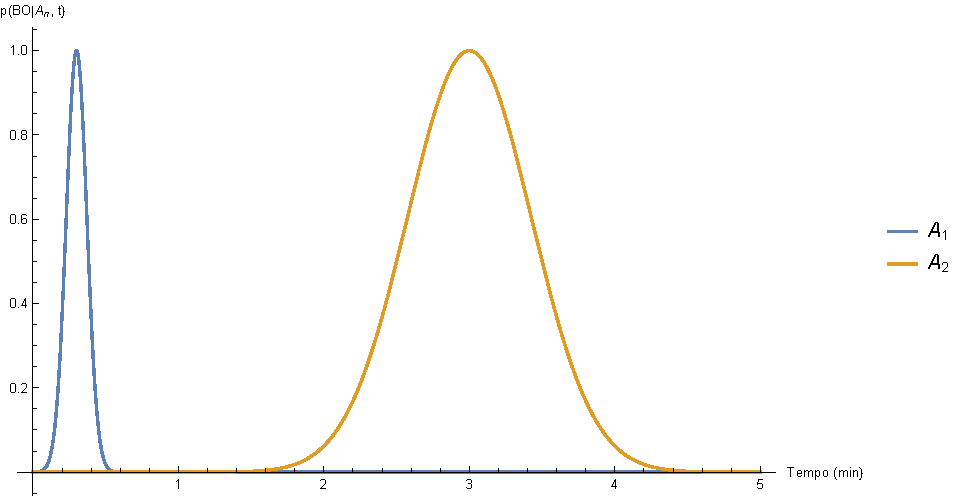
\includegraphics[width=\linewidth]{../Mathematica/Distribuicao1.pdf}
	\end{center}
\end{figure}

Na Figura \ref{fig:rev-distribuicao-exemplo} é possível observar que a primeira vez que a ação é executada, a tolerância para atraso é pequena, contudo, na segunda execução a tolerância de atraso é muito maior.

A tolerância de execução se faz necessária pois um jogador pode atrasar alguns segundos por múltiplos motivos durante o jogo, embora ele ainda esteja executando a mesma build-order.

Para uma \textit{build order} real, haverá uma distribuição de probabilidade para cada uma das ações que podem oscilar em torno de 30 a 40 dependendo da facção do jogador.

%-------------------------------------------------------------------------
		\section{Fator de \textit{branching} de um jogo de StarCraft: BroodWar}
%-------------------------------------------------------------------------
Em teoria dos jogos \todo{referencia}, \textit{branching factor} é o número de nós-filho em cada um dos nós de ações possíveis no jogo, isto é, é o número de opções que um jogador tem disponível em cada momento.

Infelizmente não há análises cientificas feitas para a complexidade de um jogo de StarCraft II, mas é possível realizar uma comparação utilizando o jogo antecessor da série, StarCraft: Brood War lançado em 1998. De acordo com \cite{weber2009data}, StarCraft: BroodWar possui um fator de branching estimado médio de $1 \times 10^6$ que, comparado à um jogo de xadrez onde a média é de 35, é um valor extremamente alto. O alto nível de complexidade força que seja utilizado um modelo probabilístico ao invés de uma análise determinista, uma vez que é impossível obter, ou sequer gerar, uma amostra para todas as possibilidades de jogos. Devido a novas mecânicas de jogo introduzidas em StarCraft II espera-se a complexidade seja superior à de seu antecessor.

%-------------------------------------------------------------------------
		\section{O Teorema de Bayes}
%-------------------------------------------------------------------------
O Teorema de Bayes relaciona a probabilidade de um evento associado à uma restrição. A definição matemática do teorema é dada pela Equação \ref{eq}:

\begin{equation}
	P(A|B) = \frac{P(B|A)P(A)}{P(B)}
\end{equation}

\noindent onde $A$ é um evento, $B$ é a restrição do evento $A$. Dessa forma, é possível determinar a probabilidade do evento $A$ ter acontecido, dado que o evento $B$ foi observado.

Em termos da análise de \textit{build orders}, pode-se aplicar o teorema da seguinte forma:

\begin{equation}
	P(BO|A, t) = \frac{P(A|BO, t)P(BO)}{P(A, t)}
\end{equation}
\noindent onde $BO$ é uma \textit{build order} qualquer que deseja-se estimar a probabilidade de estar sendo executada, dado que o jogador executou a ação $A$ no tempo $t$. Para tanto, precisa-se determinar 3 fatores:

\begin{itemize}
	\item $P(A, t)$: a probabilidade de um jogador executar a ação $A$ no instante $t$, independe da \textit{build order};
	\item $P(BO)$: a probabilidade de um jogador executar a \textit{build order} $BO$, independente da ação que o jogador está executando;
	\item $P(A|BO, t)$: a probabilidade de ter executado a ação $A$ supondo que o jogador está executando a \textit{build order} $BO$ no instante $t$;
\end{itemize}

%-------------------------------------------------------------------------
		\section{Redes Bayesianas}
%-------------------------------------------------------------------------
Uma rede Bayesiana \cite{ruggeri2007encyclopedia} é um modelo probabilístico onde uma série de eventos, com suas probabilidades condicionais, representado utilizando um grafo acíclico. Um grafo acíclico é um grafo onde não há dependências cíclicas.\todo{referencia}

\todo{explicar mais}

Dessa forma, uma \textit{build order} é vista como uma rede Bayesiana onde a transição de cada conjunto ação-\textit{build order} possui uma probabilidade.

%=========================================================================
% METODOLOGIA EXPERIMENTAL
	\chapter{Método}
%=========================================================================
Neste trabalho foi utilizado Python 2.7 como a linguagem de programação para a implementação do método. Este motivo foi guiado principalmente pelo fato da biblioteca oficial de processamento de replays oferecida pela Blizzard Entertainment, Inc. (desenvolvedor do StarCraft II) ser em Python. A biblioteca de processamento de replays oficial, \textit{s2protocol}\cite{s2protocol} é de código-fonte aberto e está disponível no GitHub. Demais códigos utilizados são parte de uma distribuição padrão do Python 2.7 ou foram desenvolvidos para o trabalho.

%-------------------------------------------------------------------------
\section{Extração dos dados}
%-------------------------------------------------------------------------

Os replays de StarCraft II são arquivos do tipo MoPAQ, um formato proprietário desenvolvido pela Blizzard Entertainment nos anos 90 para uso em seus jogos. Embora o formato seja proprietário é possível localizar na internet uma gama de implementações ou documentação desenvolvida por engenharia reversa. Um arquivo MPQ é análogo à um arquivo ZIP e contém um índice de arquivos e blocos de conteúdo. Nos \textit{replays} há uma série de \textit{stream} de eventos de jogo e neste trabalho somente será utilizado o stream chamado "Tracker Events" que são eventos cujo conteúdo é destinado para ferramentas que desejam processar os replays, ao contrário de informações úteis para a simulação do jogo. Este \textit{stream} está armazenado como "replay.tracker.events" dentro do MPQ.

O \textit{stream} de \textit{Tracker Events} foi processado utilizando uma classe em Python que extrai as seguintes informações do evento:

\begin{itemize}
	\item Nome (tipo) do evento;
	\item \textit{Game loop} do evento (o número de iteração do loop principal do jogo) \todo{explicar a conversão};
	\item ID do jogador que gerou o evento;
	\item Estrutura de dados específica de cada evento;
\end{itemize}

Dentre os vários tipos de eventos contidos neste stream, 4 destes eventos são interessantes na análise:

\begin{description}
	\item[NNet.Replay.Tracker.SPlayerStatsEvent]: contém informações sobre o estado atual do jogador. De interesse na análise: suprimento em uso pelo exército e total de suprimento disponível.
	\item[NNet.Replay.Tracker.SUnitBornEvent] evento disparado para cada unidade/estrutura criada no jogo. Este evento somente é despachado para unidades que aparecem no campo de batalha de forma "pronta", isto é, no momento em que a unidade pode ser vista pelo jogador, ela já pode ser controlada.
	\item[NNet.Replay.Tracker.SUnitInitEvent] semelhante ao evento SUnitBornEvent, mas este evento é despachado para unidades que são construídas diretamente no campo de batalha e não estão disponíveis para jogo imediatamente no instante do evento. Embora a unidade/estrutura neste evento não seja imediatamente utilizável, no método proposto, apenas o tempo em que usuário inicia a construção é considerado.
	\item[NNet.Replay.Tracker.SUpgradeEvent] evento disparado para cada melhoramento de exército realizado pelo jogador. Estes eventos são muito importantes pois podem indicar ou refinar a intenção do jogador.
\end{description}

Para o evento \textbf{SPlayerStatsEvent} são extraídas duas informações: a quantidade de suprimento utilizada pelo exército do jogador e o total de suprimento disponível para o jogador. Esta informação não é utilizada pelo método de classificação, mas é utilizada popularmente em sites de \textit{build orders} de StarCraft II, uma vez que, durante o jogo, é mais simples indexar as ações baseado no suprimento usado e total do que no instante de tempo absoluto da ação.

Para os eventos \textbf{SUnitBornEvent}, \textbf{SUnitInitEvent} e \textbf{SUpgradeEvent} descritos anteriormente, apenas uma informação é extraída: o nome da unidade, estrutura ou melhoramento feito pelo jogador. Este nome é único para cada tipo de unidade, estrutura ou melhoramento.

Uma vez que após os 6 minutos de jogo, a partida se torna reativa, ao invés de algorítmica, a sequência de eventos é truncada até os 6 minutos de jogo. Isto garante que as informações tenham menor variabilidade. \todo{explicar melhor isso}

%-------------------------------------------------------------------------
\section{\textit{Dataset} de referência}
%-------------------------------------------------------------------------
Como não há nenhum índice de replays e build-orders disponível publicamente o conjunto de replays utilizado para treinamento e validação foi classificado manualmente utilizando replays de diversos campeonatos do ano de 2016:

\begin{itemize}
	\item Intel Extreme Masters 10
	\item Intel Extreme Masters 11
	\item WCS Spring Championship 2016
	\item WCS Summer Championship 2016
	\item DreamHack ZOWIE Open Valencia
\end{itemize}
\todo{quantidade de replays em cada}

Para a classificação manual das estratégias cada replay foi assistido no jogo e classificado conforme as regras abaixo:

\begin{itemize}
	\item A composição de exército de um jogador no instante do primeiro ataque realizado por ele;
	\item Se o jogador fosse atacado por outro e tivesse mais de 8 unidades perdidas, o \textit{replay} era descartado;
	\item Caso não houvesse investida por parte dos dois jogadores até os 6 minutos de jogo, a composição de exército do jogador aos 6 minutos de jogo era classificada.
\end{itemize}

Um exército em StarCraft II pode ser composto por mais de 10 tipos de unidades diferentes, contudo isto é incomum. De forma geral, exércitos são compostos por um grande número de unidades básicas de ataque e algumas unidades de suporte. Na classificação, as unidades de suporte foram desprezadas na composição do exército. Esta regra é violada somente caso a unidade de suporte seja incomum ou trouxe um benefício significante para o jogador.

%-------------------------------------------------------------------------
\section{Treinamento}
%-------------------------------------------------------------------------

O treinamento foi realizado de forma simples: a sequência de ações para cada \textit{replay} era iterada e o tempo de execução da ação era gravado em uma lista. Uma lista separada era usada para cada repetição. Por exemplo, supondo que as \textit{build orders} $BO_1$ e $BO_2$ sejam duas amostras com o mesmo \textit{label}:

\begin{table}[H]
\centering
\caption{Um exemplo de uma \textit{build order} com as ações $A_1$ e $A_2$ ocorrendo nos tempos $t_n$.}
\label{my-label}
\begin{tabular}{|l|l||l|l|}
\hline
\multicolumn{2}{|l||}{\centering $BO_1$} & \multicolumn{2}{l|}{\centering $BO_2$} \\ \hline
\textbf{T}  & \textbf{A}  & \textbf{T}  & \textbf{A} \\ \hline
$t_1$       & $A_1$       & $t_2$       & $A_1$      \\ \hline
$t_3$       & $A_1$       & $t_4$       & $A_1$      \\ \hline
$t_5$       & $A_2$       & $t_6$       & $A_1$      \\ \hline
$t_7$       & $A_1$       & $t_8$       & $A_2$      \\ \hline
\end{tabular}
\end{table}

Dessa forma, as duas listas terão o seguinte conteúdo:

\begin{align}
\begin{split}
    T_{A_1} = \{
		&\{t_1, t_2\}, 		\\
		&\{t_3, t_4\}, 		\\
		&\{t_6, t_7\}
	\}
\end{split}
\label{eq:metodo-exemplo-vetor-tempos-a1}
\end{align}
\noindent onde $T_{A_1}$ é o vetor de tempos da execução de cada repetição da ação $A_1$ nos múltiplos \textit{replays} processados. $\{t_1, t_2\}$ representa os tempos da primeira repetição, $\{t_3, t_4\}$ da segunda e $\{t_6, t_7\}$ da terceira.

\begin{align}
\begin{split}
    T_{A_2} = \{
		&\{t_5, t_8\}
	\}
\end{split}
\label{eq:metodo-exemplo-vetor-tempos-a2}
\end{align}
\noindent onde $T_{A_2}$ é o vetor de tempos da execução de cada repetição da ação $A_2$ nos múltiplos \textit{replays} processados. Esta ação possui uma única repetição.

Seja $\mu(T_x, R)$ a média do vetor de tempo $T_x$ para a repetição $R$ e $\sigma(T_x, R)$ o desvio padrão do vetor de tempo $T_x$ para a repetição $R$, então a distribuição $p$ de probabilidade de uma ação pode ser definida como:

\begin{equation}
	p_{T_x}(t, R) = A e^{-\frac{(t-\mu(T_x, R))^2}{{\sigma(T_x, R)}^2}}
	\label{eq:metodo-funcao-distribuicao-de-probabilidade}
\end{equation}
\noindent onde $A$ é a frequência com que um par ação-repetição ocorre dentre todas as amostras de treinamento utilizadas, $\mu$ é o tempo médio de execução do par ação-repetição e $\sigma$ e o correspondente desvio-padrão.

A Equação \ref{eq:metodo-funcao-distribuicao-de-probabilidade} apresenta a função distribuição de probabilidade para uma ação. Isto é, representa a probabilidade de uma ação qualquer $A$ pertencer a uma \textit{build order} $BO_1$ dado que a ação foi executada pelo jogador no instante $t$.

\todo{explicar porque esta função}

Para o cálculo da média ($\mu$) e desvio padrão ($\sigma$) os itens internos do vetor $T_x$ são utilizados. Para o exemplo apresentado nas Equações \ref{eq:metodo-exemplo-vetor-tempos-a1} e \ref{eq:metodo-exemplo-vetor-tempos-a2}, as médias são dadas pelos vetores das Equações \ref{eq:metodo-exemplo-vetor-tempos-a1-media} e \ref{eq:metodo-exemplo-vetor-tempos-a2-media}, respectivamente:

\begin{equation}
    \mu_{A_1} = \left\{
		\frac{t_1 + t_2}{2}, 
		\frac{t_3 + t_4}{2}, 		
		\frac{t_6 + t_7}{2}
	\right\}
	\label{eq:metodo-exemplo-vetor-tempos-a1-media}
\end{equation}

\begin{equation}
    \mu_{A_1} = \left\{
		\frac{t_5 + t_8}{2}
	\right\}
	\label{eq:metodo-exemplo-vetor-tempos-a2-media}
\end{equation}

O cálculo de desvio padrão para os vetores das Equações \ref{eq:metodo-exemplo-vetor-tempos-a1} e \ref{eq:metodo-exemplo-vetor-tempos-a2} foi omitido no exemplo pois a expressão é complexa e não influencia no entendimento e um valor genérico é apresentado nas Equações \ref{eq:metodo-exemplo-vetor-tempos-a1-desvio} e \ref{eq:metodo-exemplo-vetor-tempos-a2-desvio}.\todo{reescrever}

\begin{equation}
    \sigma_{A_1} = \left\{
		\sigma_{{A_1},1}, 
		\sigma_{{A_1},2}, 	
		\sigma_{{A_1},3}
	\right\}
	\label{eq:metodo-exemplo-vetor-tempos-a1-desvio}
\end{equation}

\begin{equation}
    \sigma_{A_1} = \left\{
		\sigma_{{A_2},1}
	\right\}
	\label{eq:metodo-exemplo-vetor-tempos-a2-desvio}
\end{equation}

Neste exemplo, de forma a simplificar o cálculo, assume-se que a frequência de cada par ação-repetição é unitária.

É possível substituir os valores de média e desvio-padrão das Equações \ref{eq:metodo-exemplo-vetor-tempos-a1-media}, \ref{eq:metodo-exemplo-vetor-tempos-a2-media}, \ref{eq:metodo-exemplo-vetor-tempos-a1-desvio} e \ref{eq:metodo-exemplo-vetor-tempos-a2-desvio} na função distribuição de probabilidade da Equação \ref{eq:metodo-funcao-distribuicao-de-probabilidade}. O vetor final é denominado de "vetor de probabilidades".

Com os resultados de média (Equações \ref{eq:metodo-exemplo-vetor-tempos-a1-media} e \ref{eq:metodo-exemplo-vetor-tempos-a2-media}) e desvio padrão (Equações \ref{eq:metodo-exemplo-vetor-tempos-a1-desvio} e \ref{eq:metodo-exemplo-vetor-tempos-a2-desvio}), é possível obter um gráfico do formato da distribuição de probabilidade conforme representado nas Figuras \ref{fig:metodo-exemplo-bo-media-a1} e \ref{fig:metodo-exemplo-bo-media-a2}.

\begin{figure}[htb]
	\caption{\label{fig:metodo-exemplo-bo-media-a1} Exemplo da distribuição de probabilidade da ação $A_1$. A curva em azul representa a primeira repetição da ação (nos tempos $t_1$ e $t_2$), a curva em laranja representa a segunda repetição (nos tempos $t_3$ e $t_4$) e a curva em verde representa a terceira repetição da ação (tempos $t_6$ e $t_7$).}
	\begin{center}
	    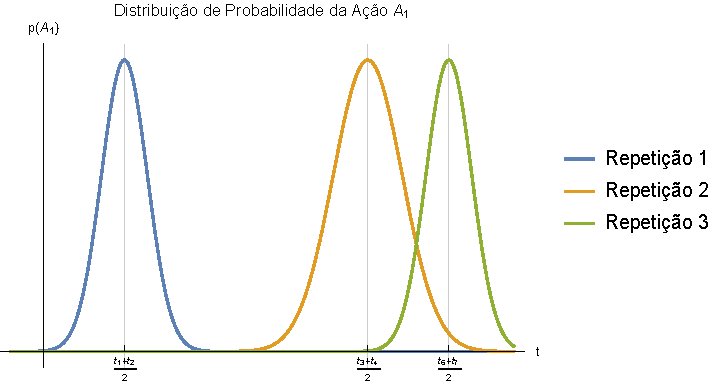
\includegraphics[width=\linewidth]{../Mathematica/Images/Exemplo_BO_Media_A1.pdf}
	\end{center}
\end{figure}

\begin{figure}[htb]
	\caption{\label{fig:metodo-exemplo-bo-media-a2} Exemplo da distribuição de probabilidade da ação $A_1$. Como a ação $A_2$ somente é executada uma única vez no exemplo, apenas uma repetição é mostrada no gráfico. A ação corresponde aos instantes de tempo $t_5$ e $t_8$.}
	\begin{center}
	    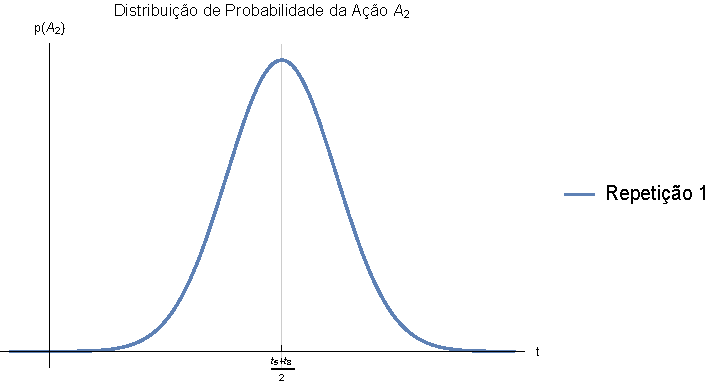
\includegraphics[width=\linewidth]{../Mathematica/Images/Exemplo_BO_Media_A2.pdf}
	\end{center}
\end{figure}

%-------------------------------------------------------------------------
\subsection{Forma Matricial}
%-------------------------------------------------------------------------
O treinamento pode ser realizado de forma matricial. Onde as colunas indicam as ações e as linhas indicam as repetições de cada ação respectiva. Dessa forma, é possível definir uma matriz de médias e desvios padrões.

Dado um conjunto de $N$ ações que podem se repetir até $M$ vezes, então, é possível definir uma matriz $M \times N$, cujos elementos são formatos pelo tempo médio de execução de cada par ação-repetição, denominada de "matriz de média do tempo de execução", expressa na Equação \ref{eq:metodo-matriz-media-simbolico}.

\newcommand{\RogielBOMatrix}[1]{
	\ensuremath{
		\left(\begin{array}{cccc}
 			{#1}_{A_1,1} & {#1}_{A_2,1} & \cdots & {#1}_{A_N,1} \\
 			{#1}_{A_1,2} & {#1}_{A_2,2} & \cdots & {#1}_{A_N,2} \\
 			\vdots 		 & \vdots 	    & \ddots & \vdots 		\\
 			{#1}_{A_1,M} & {#1}_{A_2,M} & \cdots & {#1}_{A_N,M}
		\end{array}\right)
	}
}

\begin{equation}
	\mu = \RogielBOMatrix{\mu}
	\label{eq:metodo-matriz-media-simbolico}
\end{equation}

De forma análoga a matriz de média do tempo de execução, é possível definir a "matriz de desvio padrão do tempo de execução" para os valores de desvio padrão do tempo de execução de cada par ação-repetição e a outra matriz denominada "matriz de frequência de ocorrência de repetição" que define a frequência de ocorrência de um dado par ação-repetição no conjunto de amostras observadas. A definição formal da matriz de desvio padrão do tempo de execução está apresentada na Equação \ref{eq:metodo-matriz-desvio-simbolico}. A definição formal da matriz de frequência de repetição está apresentada na Equação \ref{eq:metodo-matriz-frequencia-simbolico}.

\begin{equation}
	\sigma = \RogielBOMatrix{\sigma}
	\label{eq:metodo-matriz-desvio-simbolico}
\end{equation}

\begin{equation}
	F = \RogielBOMatrix{F}
	\label{eq:metodo-matriz-frequencia-simbolico}
\end{equation}


Substituindo-se as matrizes de média e desvio padrão do tempo de execução e de frequência de ocorrência de repetição, Equações \ref{eq:metodo-matriz-media-simbolico}, \ref{eq:metodo-matriz-desvio-simbolico} e \ref{eq:metodo-matriz-frequencia-simbolico}, respectivamente, na função de distribuição de probabilidade dada pela Equação \ref{eq:metodo-funcao-distribuicao-de-probabilidade}, é possível construir um vetor de probabilidade. Todas as operações entre matrizes são realizadas utilizando operadores de Hadamard\todo{referencia} ou operações termo-a-termo.

Por convenção matemática, e evitar um problema de indeterminação no cálculo de probabilidade associada, uma ação cuja repetição não ocorre nas amostras encontradas, deve ter o valor de média não-nulo e o valor de desvio padrão deve ser infinito. Por convenção, neste trabalho utiliza-se o valor de média $0.0$. Este escolha foi feita para que a função distribuição de probabilidade seja avaliada com valor $1.0$ para ações inexistentes na amostra de treinamento, independente da ação ser executada pelo jogador numa \textit{build order} utilizada no processo de classificação.

\newcommand{\RPME}[4]{
	\ensuremath{
		{#1} e^{-\frac{(#4-{#2})^2}{{{#3}}^2}}
	}
}
\newcommand{\RPMGE}[1]{
	\RPME{F_{{#1}}}{\mu_{{#1}}}{\sigma_{{#1}}}{t_{{#1}}}
}


\begin{equation}
	p(t) = \left(
		\begin{array}{cccc}
			\RPMGE{A_1,1} & \RPMGE{A_2,1} & \cdots & \RPMGE{A_N,1} \\
 			\RPMGE{A_1,2} & \RPMGE{A_2,2} & \cdots & \RPMGE{A_N,2} \\
 			\vdots 	  	  & \vdots 	  	  & \ddots & \vdots 	       \\
 			\RPMGE{A_1,M} & \RPMGE{A_2,M} & \cdots & \RPMGE{A_N,M}
		\end{array}
	\right)
	\label{eq:metodo-matriz-probabilidade-simbolico}
\end{equation}
\noindent onde $t$ é uma matriz que indica o tempo de execução dos pares ação-repetição de uma \textit{build order} que se deseja classificar.

%-------------------------------------------------------------------------
\section{Classificação}
%-------------------------------------------------------------------------
O processo de classificação é realizado de forma independente para cada \textit{label} (\textit{build order}) utilizado no processo de treinamento. Os valores de probabilidade para cada par de ação-tempo de um \textit{replay} são multiplicados e o valor final determina a semelhança de uma \textit{build order} treinada e a executada.

Considerando-se o exemplo anterior, é possível aplicar o instante de execução de cada ação do jogador no vetor de ações correspondente e obter a probabilidade de que uma ação qualquer $A$. Dessa forma, a probabilidade total de que um conjunto de ações seja parte de uma \textit{build order} qualquer é dada pela Equação \ref{eq:metodo-exemplo-classificacao-produto}:

\begin{equation}
	p_{BO} = \prod_{n,i} p(BO|A_{(n,i)}, t)
	\label{eq:metodo-exemplo-classificacao-produto}
\end{equation}
\noindent onde $n$ indica o tipo da ação, $i$ a sua repetição e $p(BO|A_{(n,i)}, t)$ é a probabilidade de que a ação seja parte de uma build order $BO$ dado que $A_{(n,i)}$ foi executada no instante de tempo $t$, conforme a Equação \ref{eq:metodo-funcao-distribuicao-de-probabilidade}.

%-------------------------------------------------------------------------
\subsection{Forma Matricial}
%-------------------------------------------------------------------------
Dada a matriz de probabilidades de uma \textit{build order} treinada, conforme a Equação \ref{eq:metodo-matriz-probabilidade-simbolico}, a probabilidade final de uma \textit{build order} treinada é dada pela redução da matriz através da operação de multiplicação de seus termos, conforme Equação \ref{eq:metodo-matriz-reducao}.

\begin{equation}
	p_{BO} = \prod_{i,j} p(t)_{ij}
	\label{eq:metodo-matriz-reducao}
\end{equation}
\noindent onde $i$ e $j$ são respectivamente as linhas e as colunas das matrizes de probabilidade e de tempo de execução da \textit{build order} a ser classificada, $t$ é a matriz de tempo de execução da \textit{build order} para ser classificada, $p$ é a matriz de probabilidades de uma \textit{build order} qualquer $BO$ e $p_{BO}$ é a probabilidade reduzida da matriz $p$ cujo valor é equivalente à operação da Equação \ref{eq:metodo-exemplo-classificacao-produto}.

%-------------------------------------------------------------------------
\section{Comparação}
%-------------------------------------------------------------------------
Para realizar a comparação entre \textit{build orders} é feita uma tabela que compara a taxa de vitória de cada \textit{build order} contra a \textit{build order} do oponente.

%=========================================================================
% RESULTADOS E DISCUSSÕES
	\chapter{Resultados e Discussões}
%=========================================================================

No processo de treinamento, é extraído a sequência de construção de cada jogador (a \textit{build order}), calculadas estatísticas de primeira ordem (média e desvio padrão) e a frequência de cada par ação-repetição em relação ao conjunto de replays correspondentes a mesma \textit{build order}.

A Figura \ref{fig:resultados-protoss-immortal-gateway} apresenta a \todo{}

\begin{figure}[htb]
	\caption{\label{fig:resultados-protoss-immortal-gateway} Forma gráfica de distribuição estatística de uma ação \textit{Gateway} e suas repetições}
	\begin{center}
	    \includegraphics[width=\linewidth]{{"../Classifier/Graphs/Protoss/Adept Immortal"}/Gateway.png}
	\end{center}
\end{figure}

Observa-se que a frequência de ocorrência das repetições no \textit{dataset} de treinamento é decrescente. Isto é uma consequência do método escolhido para classificação. A primeira execução de uma ação, irá, independentemente do tempo em que for executada, considerada como a primeira repetição. A redução da frequência tem duas causas principais:

\begin{description}
	\item[Alteração da estratégia do jogador]: um jogador pode ter escolhido uma estratégia levemente diferente devido ao contexto do jogo ou em resposta à \textit{build order} do oponente;
	\item[Ações opcionais]: algumas ações podem ser opcionais e somente são executadas em alguns mapas. 
\end{description}

Há uma tendência no desvio-padrão e variância do tempo de execução do par ação-repetição de crescerem ao decorrer da partida. Os principais motivos deste crescimento é a incapacidade de jogadores humanos executarem as ações de forma perfeita e sem qualquer variabilidade. Este fator é agravado com a característica da "árvore tecnológica" onde algumas ações possuem dependências tecnológicas em outras anteriores. Embora a tendência seja visível na maior parte das ações, ainda é possível que ela reduza em alguns casos específicos.

Um exemplo onde o desvio padrão reduz de forma significante é visível na Figura \todo{} onde a primeira repetição possui um desvio padrão significantemente maior ao da segunda repetição. Este comportamento é esperado quando a primeira ação é considerada opcional e incorre num erro onde a primeira repetição deveria ter frequência menor que a segunda. Infelizmente, devido à forma de como o método de separação foi estabelecido, não é possível evitar este efeito.

\todo{figura adept}

O resultado da classificação é validado utilizando um método de validação cruzada onde o primeiro item da lista de \textit{replays} é removido do treinamento e utilizado como item de validação.

%=========================================================================
% CONCLUSÃO
	\chapter{Conclusões}
%=========================================================================


%=========================================================================
% PROPOSTA DE TRABALHOS FUTUROS
	\chapter{Propostas de Trabalhos Futuros}
%=========================================================================
\begin{itemize}
	\item Utilização de um refinamento utilizando ações-chave
\end{itemize}

%=========================================================================
% REFERÊNCIAS BIBLIOGRÁFICAS
	\postextual
	\bibliography{Referencias.bib}
%=========================================================================

%%=========================================================================
%% APÊNDICES
%\begin{apendicesenv}
%\partapendices
%%=========================================================================
%
%\end{apendicesenv}
%
%%=========================================================================
%% ANEXOS
%	\begin{anexosenv}
%	\partanexos
%%=========================================================================
%
%
%%-------------------------------------------------------------------------
%\end{anexosenv}

\end{document}
